\section{Introduction}

Big Data is a portfolio of technologies that were designed to store, manage and analyze data that is too large to fit on a single machine while accommodating for the issue of growing discrepancy between capacity, throughput and latency.

\begin{figure}[h]
	\centering
	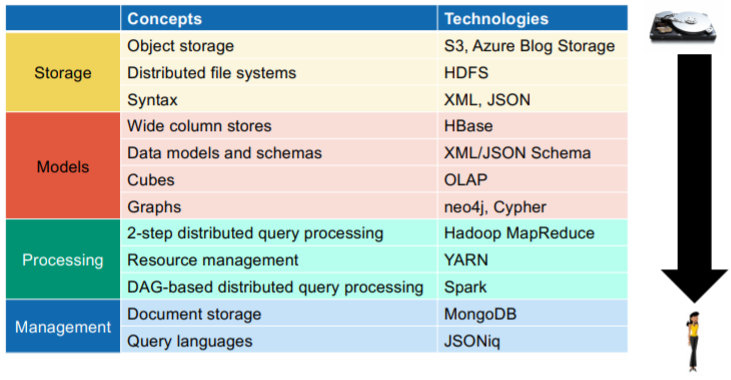
\includegraphics[scale=0.8]{images/1-overview.PNG}
	\caption{Lecture overview.}
	\label{fig:overview}
\end{figure}

\begin{figure}[h]
	\centering
	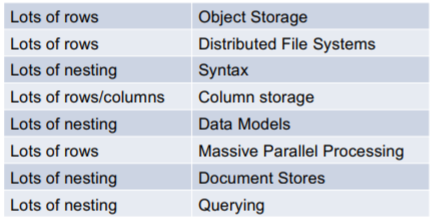
\includegraphics[scale=0.7]{images/1-scale.PNG}
	\caption{Scaling up.}
	\label{fig:scale}
\end{figure}

\begin{figure}[h]
	\centering
	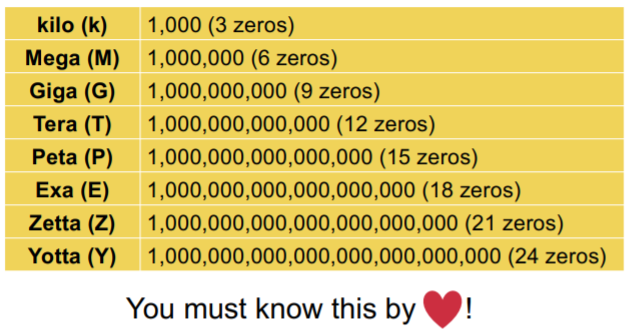
\includegraphics[scale=0.5]{images/1-prefixes.PNG}
	\caption{Prefixes (International System of Units).}
	\label{fig:prefix}
\end{figure}

\begin{figure}[h]
	\centering
	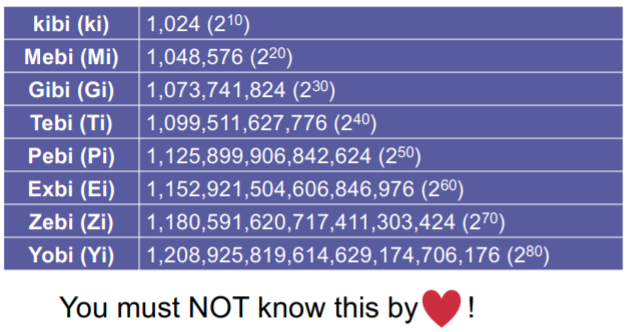
\includegraphics[scale=0.5]{images/1-prefixesb2.PNG}
	\caption{Prefixes for base 2.}
	\label{fig:prefix2}
\end{figure}

\subsection{Concepts}

\paragraph{Table}
A table in a relational model is also called a collection.

\paragraph{Attribute}
An attribute in a relational model is also called a column, field or property.

\paragraph{Primary Key}
The identifying attribute is also called row ID or name of a row.

\paragraph{Row}
A row in a relational model is also called a business object, item, entity, document or record.

\paragraph{Relational Algebra}
A table in a relational model is a relation $R$. It is made of a set of attributes and an extension (set of tuples). (String to Value mappings)

$$
\text{Attributes}_R \subseteq \mathbb{S}
$$

$$
\text{Extension}_R \subseteq \mathbb{S} \mapsto \mathbb{V}
$$

\paragraph{Tabular Integrity}
Each row of a table has the same schema and no empty values.

\paragraph{Atomic Integrity (1st Normal Form)}
The domain of each attribute contains only atomic (indivisible) values and the value of each attribute contains only a single value from that domain. E.g. a column cannot include entire table as values.

\paragraph{Domain Integrity}
Each attribute has a specified data type (domain) and its values are from that domain. E.g. a Boolean column contains only true and false (no zeros and ones).

\paragraph{SQL vs. NoSQL}
SQL has all the integrity properties mentioned above while NoSQL (not relational) can break any or even all of those.

\paragraph{Relational Queries}
We can have:
\begin{itemize}
    \item \textbf{Set:} Union, intersection, subtraction.
    \item \textbf{Filter:} Selection (subset of rows) and projection (subset of columns).
    \item \textbf{Renaming:} Relation and attribute renaming.
    \item \textbf{Binary:} Cartesian product, natural join, theta join.
    \item \textbf{Grouping:} Make groups of the same values in a specific column and summarize the groups items (sum, avg, etc.).
\end{itemize}


\paragraph{Normal Forms / Database Normalization}
A relational database can be structured to be in accordance to one or a set of normal forms. A normalized database reduces data redundancy and improves data integrity. For data to be consistent, we need to avoid:
\begin{itemize}
    \item \textbf{Update anomalies:} A row with the same identifier has two different values for the same attribute. Happens if there are too many places to update (and they're not linked).
    \item \textbf{Deletion anomalies:} The deletion of unwanted information causes desired information to be deleted as well. Happens if too much information is stored in a single record. 
    \item \textbf{Insertion anomalies:} New data cannot be inserted since some information is not available yet. Happens if a new record is missing a value for one of the necessary attributes (new prof, no assigned course yet).
\end{itemize}



\paragraph{0NF / UNF}
Any table that is not normalized.

\paragraph{1NF}
Each field contains a single value and reach row is unique (and can be identified by some primary key).

\paragraph{2NF}
Relation is in 1NF and no non-key attribute is dependent on only a subset of any candidate key.

\paragraph{3NF}
Relation is in 2NF and ...

%TODO maths and stuff? How important is it?


\paragraph{Transactions and ACID}
A transaction is a set of operations. It is correct if it follows the ACID principles:
\begin{itemize}
    \item \textbf{Atomicity:} Each transaction is atomic, i.e. it is either applies as a whole or undone.
    \item \textbf{Consistency:} A Transaction starts and ends in a consistent state (if it commits).¨
    \item \textbf{Isolation:} Intermediate states of a transaction are not seen by any other transactions. Transactions feel like they're alone.
    \item \textbf{Durability:} Committed updates do not disappear again (in case of failures).
\end{itemize}

\paragraph{Index}

\paragraph{OLTP vs. OLAP}

\paragraph{RDBMS vs. Big Data}
%TODO stack image, different concistency constraints, ACID vs. CAP, new concepts (lec 3)


\subsection{SQL Brush Up}

%TODO SQL cheat sheet





\subsection{Exercises}

\subsubsection{SQL Brush Up}